\documentclass{exam}
\usepackage{../../mypackages}
\usepackage{../../macros}

\setlength{\parindent}{0pt}

\title{Devoir sur table N°1 \par 
Généralités sur les matériaux \& L'atome}
\author{N. Bancel}
\date{9 Octobre 2024}

\begin{document}

\textbf{Collège Lycée Suger}
\hfill
\textbf{Physique-Chimie} \\

\textbf{Année 2024-2025}
\hfill
\textbf{1ère STD2A} \par

{\let\newpage\relax\maketitle}
%\maketitle

\begin{center}
  \textbf{\textcolor{blue}{Durée du devoir : 2 heures}} \par
  \vspace{1em}
  \textbf{\textcolor{red}{La calculatrice n'est pas autorisée}}
\end{center}

\begin{tcolorbox}[colback=gray!10!white, colframe=gray, title=Note importante]
  \itshape{Toutes les réponses doivent être justifiées.
  La qualité et la précision de la rédaction seront prises en compte dans la notation des copies.
  Il est permis d'admettre le résultat de certaines questions pour ne pas rester bloqué, en prenant soin d'indiquer sur la copie les résultats admis. \par
  \vspace{1em}
  Exemples :
  \begin{itemize}
    \item Si vous connaissez par coeur le schéma de Lewis d'un atome mais n'êtes plus capable de le justifier, vous pouvez utiliser votre schéma appris par coeur pour résoudre les questions suivantes 
    \item Si une question demande d'avoir la réponse à la question précédente, vous pouvez expliquer comment vous auriez résolu le problème si vous aviez réussi la question précédente
  \end{itemize}
  }
\end{tcolorbox}

\section*{Exercice 1 [4 points] Les matériaux - Cours}

\begin{questions}
\question[1] Lister les 3 grandes familles de matériaux, et en donner une définition rapide.
\question[1] Dresser un tableau des 3 familles, placer les matériaux suivants dans la catégorie à laquelle ils appartiennent : 
  
\begin{enumerate}[noitemsep]
  \item Diamant
  \item Cuir
  \item Laine
  \item Bois 
  \item Porcelaine
  \item Bronze
  \item Matières plastiques
  \item Cuivre
  \item Laine 
  \item Verre
  \item Fer
  \item Sable 
  \item Coton 
\end{enumerate}

\question[1] Quelle est la différence entre un métal pur et un alliage ? Quelle est la composition du bronze ?

\question[1] Le choix d'un matériau se fait en fonction de ses propriétés \textbf{chimiques}, \textbf{physiques}, et \textbf{mécaniques}. Citer au moins 4 propriétés de matériaux, et expliquer la nature de cette propriété (est-ce que c'est une propriété chimique, physique, ou mécanique ?)

\end{questions}

\section*{Exercice 2 [5 points] Structural Stripes}

\begin{minipage}[c]{0.45\linewidth}
  \begin{figure}[H]
    \centering
    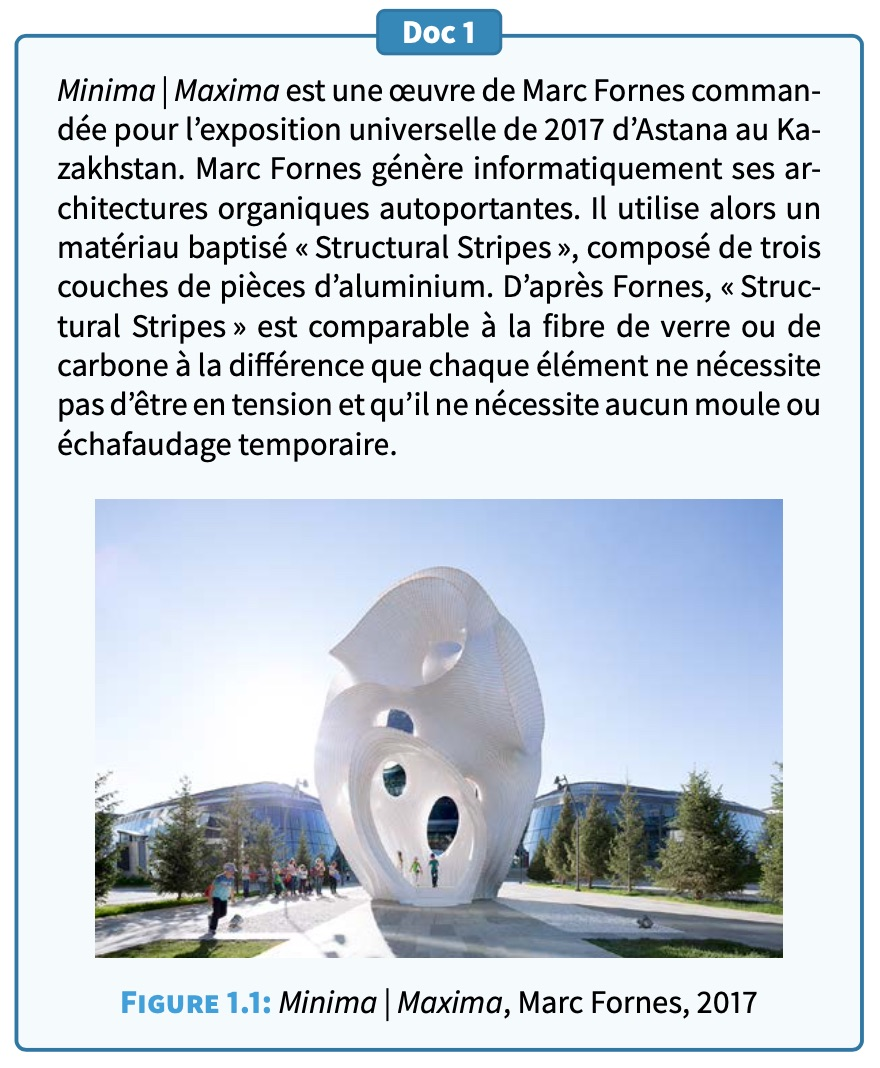
\includegraphics[width=0.9\linewidth]{dst1_fig1.jpg}
  \end{figure}

  \begin{figure}[H]
    \centering
    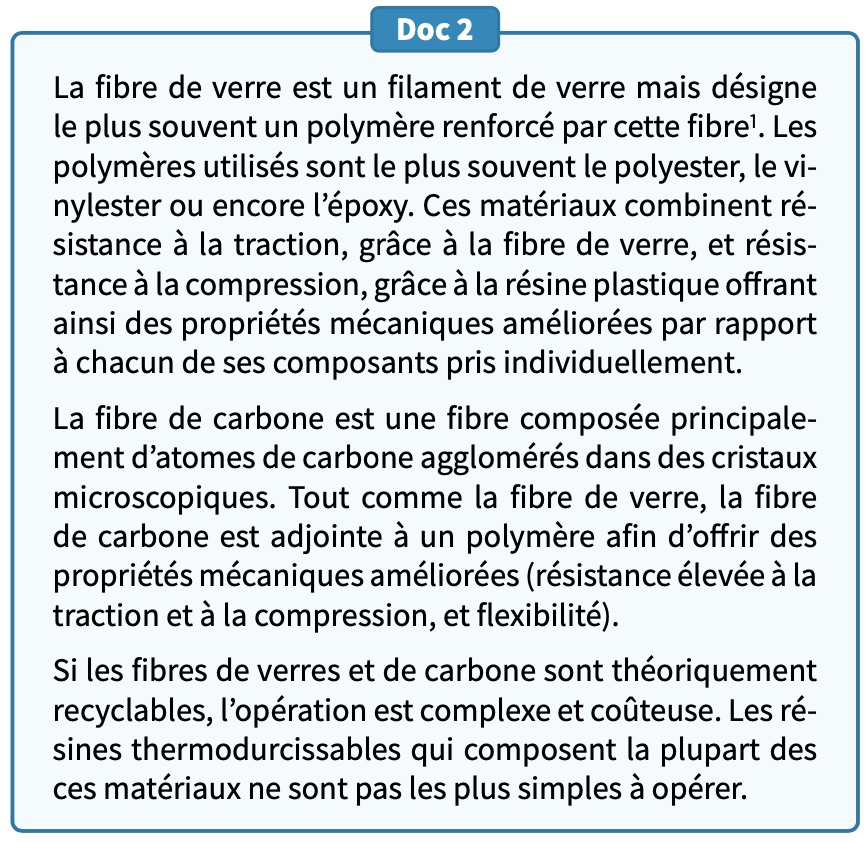
\includegraphics[width=0.9\linewidth]{dst1_fig2.jpg}
  \end{figure}
  
  \end{minipage} 
  %\hfill
  \begin{minipage}[c]{0.45\linewidth}
    \begin{figure}[H]
      \centering
      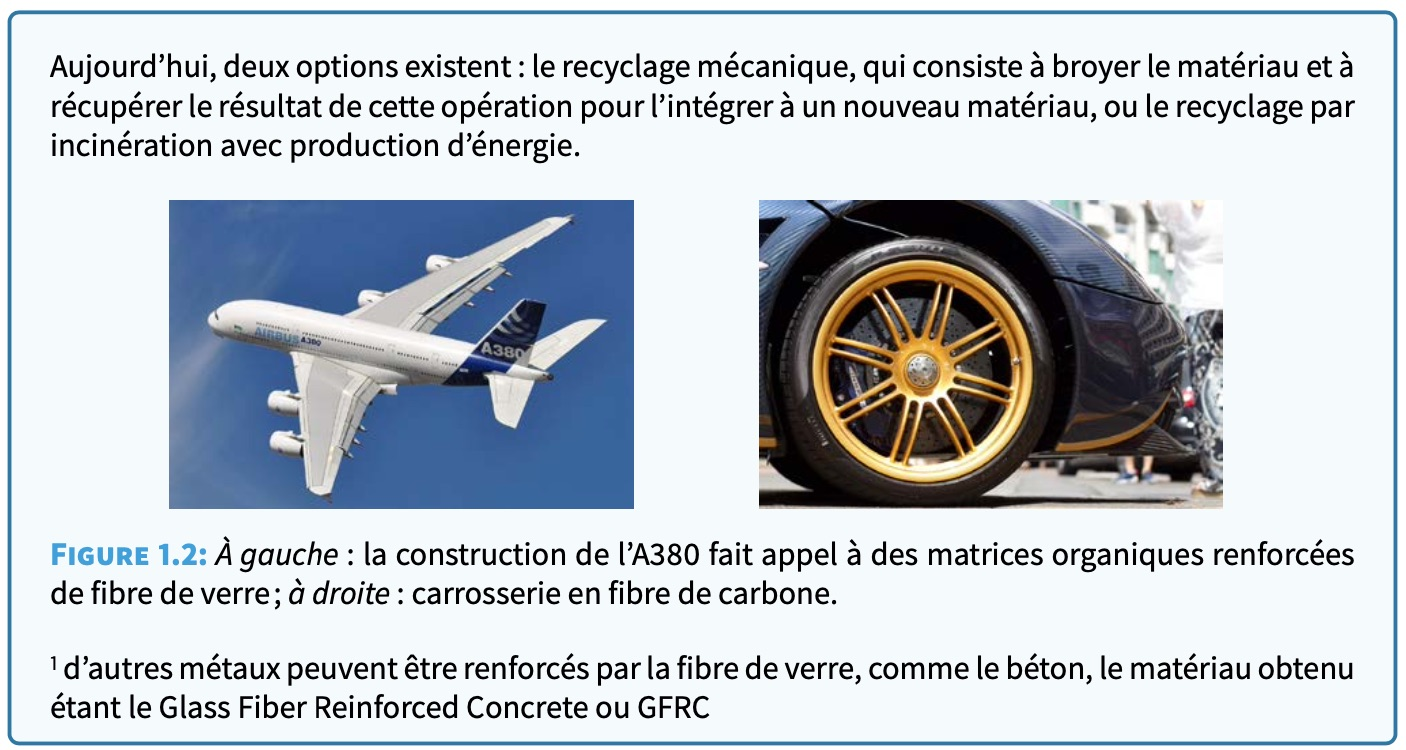
\includegraphics[width=1.5\linewidth]{dst1_fig3.jpg}
    \end{figure}

    \begin{figure}[H]
      \centering
      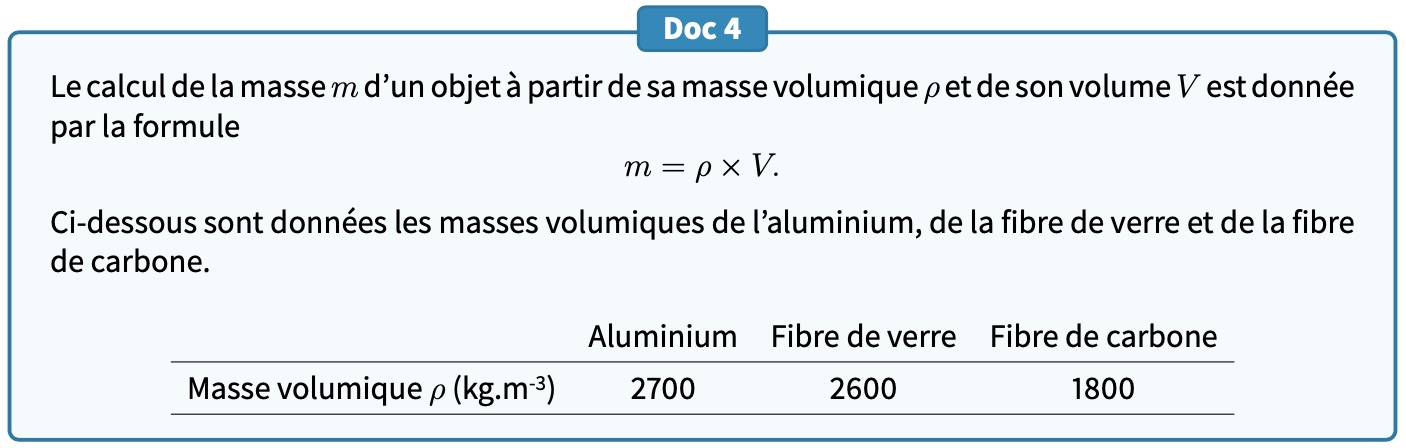
\includegraphics[width=1.5\linewidth]{dst1_fig4.jpg}
    \end{figure}
  \end{minipage}

\vspace{1em}
A partir des documents précédents, et grâce à vos connaissances personnelles, répondre aux questions suivantes : 

\begin{questions}

\question[1] Qu'est ce qu'un matériau composite, et de quoi est-il constitué (on donnera si possible une définition de chaque composant)
\question[0.5] À quelle catégorie de matériau appartiennent la fibre de verre et la fibre de carbone ? Justifier.
\question[0.5] À quelle catégorie de matériau appartient "Structural Stripes" ? Justifier.
\question[1] Quels sont les avantages de "Structural Stripes" comparativement à la fibre de verre ou de carbone ? Justifier
\question[2] Le volume total de l'oeuvre de Marc Fornes étant de $12m^3$, calculer le poids de la structure.

\end{questions}

\section*{Exercice 3 [8 points] L'atome}

\begin{tcolorbox}[colback=gray!10!white, colframe=black, title=Note importante]
  Dans la question 2, il est attendu d'expliquer au début de la question la méthode / la démarche pour arriver au schéma de Lewis, et à quoi sert chaque étape intermédiaire.
  Il ne sera pas nécessaire de ré expliquer dans le détail la démarche pour chaque atome si elle est bien expliquée en début de question. 
\end{tcolorbox}

\begin{questions}

\question[1] Donner la définition de (1) la règle du duet et de l'octet et (2) celle d'un gaz noble
\question[4] Pour chacun des atomes suivants, donner : 

\begin{itemize}[noitemsep]
  \item Sa configuration électronique (justifier comment on trouve le nombre d'électrons)
  \item Citer quelle est sa couche de valence, et son nombre d'électrons de valence 
  \item Dessiner son schéma de Lewis, en prenant bien soin de représenter les doublets non liants, et les électrons célibataires. 
\end{itemize}

\textbf{Liste des atomes}

\begin{itemize}[noitemsep]
  \item Carbone (\ce{C}) // Numéro atomique : $Z = 6$
  \item Argon (\ce{Ar}) // Numéro atomique : $Z = 18$
  \item Azote (\ce{N}) // Numéro atomique : $Z = 7$
  \item Hydrogène (\ce{H}) // Numéro atomique : $Z = 1$
  \item Oxygène (\ce{O}) // Numéro atomique : $Z = 8$
\end{itemize}

\question[3] En déduire la représentation de Lewis des molécules suivantes (une justification est demandée) : 

\begin{itemize}[noitemsep]
  \item Eau (\ce{H2O})
  \item Méthane (\ce{CH4})
  \item Ammoniac (\ce{NH3})
  \item Dioxyde de carbone (\ce{CO2})
\end{itemize}

\end{questions}

\section*{Exercice 4 [3 points] Masse volumique}

La masse volumique du sable est de \SI{1850}{kg/m^3} en moyenne. Pour un chantier, une entreprise de maçonnerie a besoin de \SI{50}{tonnes} de sable.

\begin{tcolorbox}[colback=blue!10!white, colframe=blue!70!black, title=Indication]
  Les résultats des 2 fractions suivantes pourraient aider à la résolution de l'exercice. Attention : cela ne veut pas dire que la fraction correspond exactement au calcul qui doit être fait dans l'exercice. \par
  \vspace{1em}
  Calcul 1 : $\frac{50}{18.5} \approx 2.702$ \par 
  \vspace{1em}
  Calcul 2 : $\frac{60.2}{21} \approx 2.866$
\end{tcolorbox}

\begin{questions}  
\question[2] L'entreprise peut-elle transporter tout le sable dans un camion benne de \SI{21}{m^3} ? Pourquoi ?
\question[1] Si l'on suppose que le 1er camion a été intégralement rempli de sable, quel est le \% de remplissage du 2ème camion ?
\end{questions}

\end{document}







